\section{Fritlegemediagram og analyse af pendul}\label{sec:sec_fritlegemediagram}

\begin{wrapfigure}{r}{0.4\textwidth}
	\centering
	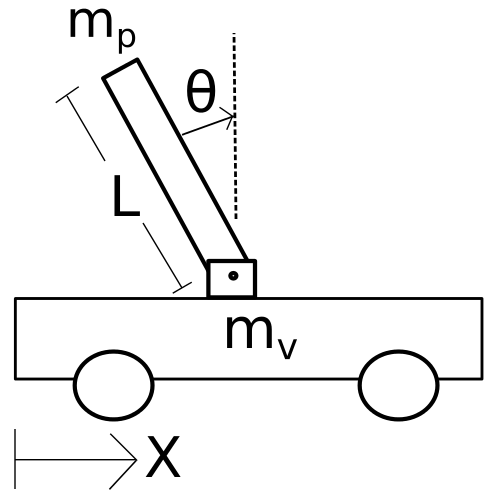
\includegraphics[width=.3\textwidth]{billeder/pendul_vogn.png}
	\caption{Simpel model af pendul og vogn.}
	\label{fig:pendul_vogn}
\end{wrapfigure}
\FloatBlock

Det inverterede pendul er monteret på en vogn med hjul, som vist i figur \ref{fig:pendul_vogn}.
Således er det muligt at flytte vognen samtidig med at der er fri bevægelse af pendulet rundt om pendulets rotations punkt, der er fastgjort på vognen.
Der er således kun tale om én-dimensional bevægelse af vognen.

Det vælges at analysere pendulet og vognen hver for sig.
Pendulet anses som en masseløs stang hvor massen er fastgjort for enden af stangen. 
Således angiver $T$ den trækkraft der er mellem vogn og pendul.
\begin{figure}
	\centering
	\subbottom[]{%
		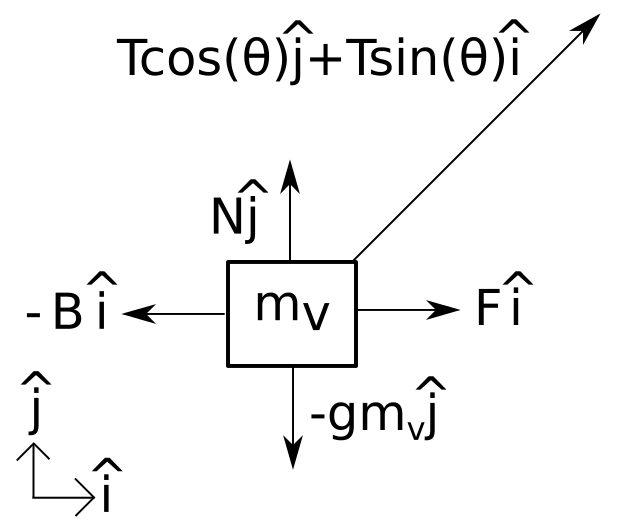
\includegraphics[width=.39\textwidth]{billeder/fridiagram_vogn.png}
		\label{fig:fridiagram_vogn}}
	\subbottom[]{%
		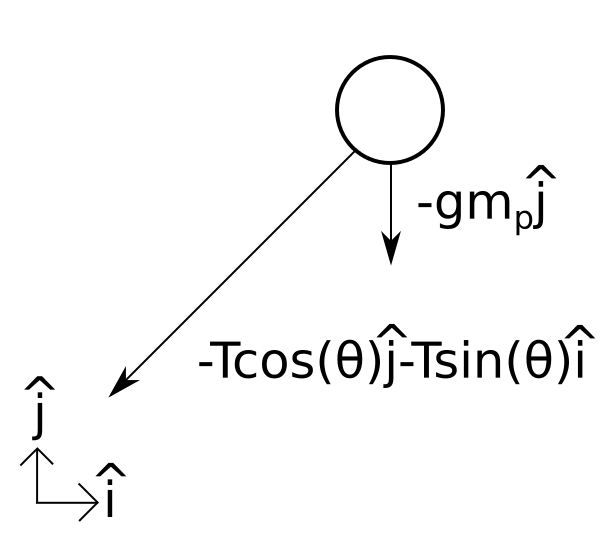
\includegraphics[width=.39\textwidth]{billeder/fridiagram_pendul.png}
		\label{fig:fridiagram_pendul}}
	\caption[Frit-legeme digrammer af vogn og pendul]{Frit-legeme diagrammer af henholdsvis vogn (a) og pendul (b).}
	\label{fig:fridiagrammer}
\end{figure}

Opsummering af kræfter på vognen som ses i frit-legeme diagrammet i figur \ref{fig:fridiagram_vogn}. 
\begin{alignat}{3}
&\hat{i} : \quad && F_c + T sin{\theta} && = m_v \ddot{x} \label{eq:vogn_x}\\
&\hat{j} : \quad && -g m_v + N && = 0 
\end{alignat}

Opsummering af kræfter på pendulet som ses i frit-legeme diagrammet i figur \ref{fig:fridiagram_pendul}.
\begin{alignat}{3}
&\hat{i} : \quad &&-T sin{\theta} &&= m_p a_{px}\label{eq:apx}\\
&\hat{j} : \quad &&-T cos{\theta} - m_p g &&= m_p a_{py}\label{eq:apy} 
\end{alignat}

\begin{wrapfigure}{r}{0.4\textwidth}
	\centering
	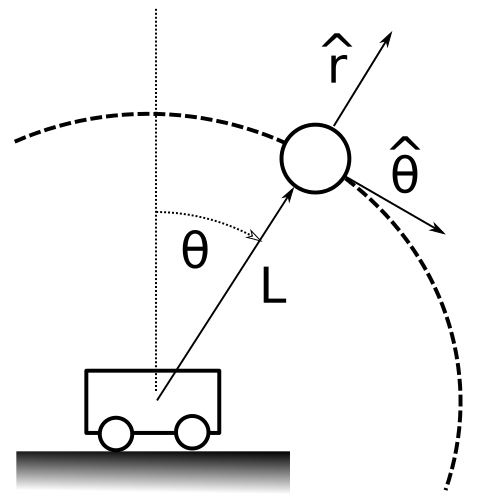
\includegraphics[width=.3\textwidth]{billeder/pendul_vogn_polaer.png}
	\caption{Retnings angivelse for polær koordinater på pendul.}
	\label{fig:pendul_vogn_polaer}
\end{wrapfigure}

Den relative acceleration af pendulet udledes i polær koordinater med retnings reference som angivet i figur \ref{fig:pendul_vogn_polaer}. 
\begin{align}
\vec{a}_p &= \vec{a}_v + \vec{a}_{p/v} \\
&= \ddot{x} \hat{i} + \left( L\ddot{\theta}\hat{\theta} - L\dot{\theta}^2\hat{r} \right)
\end{align}

Accelerationsvektoren $\vec{a}_p$, for pendulet omskrives nu fra polær-koordinator til kartesiske koordinator  
\begin{align}
\vec{a}_p &=  \ddot{x} \hat{i} 
				+ L\ddot{\theta} \left( \cos{\theta}\hat{i} - \sin{\theta}\hat{j} \right) 
				- L\dot{\theta}^2 \left( \sin{\theta}\hat{i} + \cos{\theta}\hat{j} \right) \label{eq:ap}
\end{align} 

Accelerationen for pendulet, $\vec{a}_{px}$ og $\vec{a}_{py}$, i ligning \ref{eq:apx} og \ref{eq:apy} kan nu erstattes, med den relative acceleration fundet i ligning \ref{eq:ap}
\begin{align}
-T\sin{\theta} &= m_p \left( \ddot{x} + L\ddot{\theta}\cos{\theta} - L\dot{\theta}^2\sin{\theta} \right)  \label{eq:pendul_x2}\\
-T\cos{\theta} - m_p g &=  -m_p \left( L\ddot{\theta}\sin{\theta} + L\dot{\theta}^2\cos{\theta}  \right) \label{eq:pendul_y2}
\end{align} 

Trækkræfter $T$ fjernes fra pendul ligningerne \ref{eq:pendul_x2} og \ref{eq:pendul_y2} ved gensidig at gange med $-\cos{\theta}$ og $\sin{\theta}$. 
\begin{align}
T\sin{\theta}\cos{\theta} &=   -m_p \cos{\theta} \left( \ddot{x} + L\ddot{\theta}\cos{\theta} - L\dot{\theta}^2\sin{\theta} \right) \label{eq:pendul_x3} \\
-T\cos{\theta}\sin{\theta} - m_p g &=  -m_p \sin{\theta} \left( L\ddot{\theta}\sin{\theta} + L\dot{\theta}^2\cos{\theta}\right) \label{eq:pendul_y3}
\end{align}

Ligning \ref{eq:pendul_x3} og \ref{eq:pendul_y3} adderes
\begin{align}
-m_p g \sin{\theta}    &= - m_p \ddot{x}\cos{\theta}
						- m_p L\ddot{\theta}\cos^2\theta\
						\hcancel[red]{+ m_p L \dot{\theta}^2\cos{\theta}\sin{\theta}}\\
					   &\quad - m_p L\ddot{\theta}\sin^2\theta\
					    \hcancel[red]{- m_p L \dot{\theta}^2\cos{\theta}\sin{\theta}} \\
					   &=- m_p \cos{\theta}\ddot{x} - m_p L \ddot{\theta} \left(\sin^2 \theta \cos^2 \theta \right) \\
					   &=- m_p \cos{\theta}\ddot{x} - m_p L \ddot{\theta} \label{eq:pendul_mellem}
\end{align}

I ligning \ref{eq:vogn_x} fjernes $T$ ved at substituere med ligning \ref{eq:pendul_x2}
\begin{align}
F_c - m_p \ddot{x} - m_p L\ddot{\theta}\cos{\theta} + m_p L\dot{\theta}^2\sin{\theta} &= m_v \ddot{x} \Leftrightarrow \\
F_c - m_p L\ddot{\theta}\cos{\theta} + m_p L\dot{\theta}^2\sin{\theta} &= (m_v + m_p)  \ddot{x} \label{eq:vogn_mellem}
\end{align}

Ligningerne af det fysiske system for pendul og vogn fremstår i nu i \ref{eq:pendul_mellem} og \ref{eq:vogn_mellem}. Disse to ligninger er ikke lineære. En forudsætning for at kunne gennemføre en linearisering er at antage, at udefrakommende påvirkninger til systemet er så små, at små forstyrrelser kun give anledning til små ændringer af vinkelen $\theta$ og en approksimmering kan antages som
\begin{align}
\sin{\theta} \approxeq \theta \quad og \cos{\theta} \approxeq 1
\end{align} 

Ligeledes kan udtrykket $\dot{\theta}^2$ reduceres til
\begin{align}
\dot{\theta}^2 = \left( \dfrac{d}{dt}\theta \right)^2 =  \left( \dfrac{d}{dt}\sin{\theta} \right)^2 = \left(\cos{\theta}\right)^2 \approxeq (1)^2 = 1
\end{align}

Det ønskes at få et udtryk der forbinder position $x$ med vinklen $\theta$ for pendulet, så ligning \ref{eq:pendul_mellem} forkortes. Pendulets masse $m_p$ forkortes også bort. 
\begin{align}
-m_pg\theta &= -m_p\ddot{x}-m_p L \ddot{\theta} \Leftrightarrow\\
\ddot{x} &= g \theta -L \ddot{\theta} \label{eq:pendul_lin}
\end{align}

Nu tages \ref{eq:pendul_lin} og indsættes i ligning \ref{eq:vogn_mellem}
\begin{align}
F_c - m_p L\ddot{\theta} + m_p L\theta &= (m_v + m_p)(g \theta -L \ddot{\theta})  \\
F_c  - m_p L\ddot{\theta} + m_p L\theta &= m_v g \theta +  m_p g \theta - m_v L \ddot{\theta} - m_p L \ddot{\theta}
\end{align}

I ovenstående udtryk, erstattes $F_c = ma_v$ for og reduceres
\begin{align}
m a_v - \hcancel[red]{ m_p L\ddot{\theta}} + m_p L\theta &= (m_v + m_p) g \theta - m_v L \ddot{\theta} - \hcancel[red]{ m_p L\ddot{\theta}} \Leftrightarrow \\
m_v L \ddot{\theta} - m g \theta &= - m_p L\theta -m a_v \label{eq:system_final}
\end{align} 

Ligning \ref{eq:system_final} er således den endelige beskrivelse af pendul og vogn hvori systemets overførelses funktion kan findes.
På højre side ses de eksterne forstyrrelser. 
$m_pL\theta $ er påvirkningen af en lille ændring af pendulet, og $m a_v$ er en ændring i vognens acceleration.